\chapter{Background container technology}
\label{ch:back}

The background chapter provides the necessary knowledge about containers in a structured form.
Containerization is classified and described superficially. Then the containerization core concepts can be discussed in more detail.
Practical examples are given to demonstrate these concepts.
Afterwards basic knowledge of union file systems is provided in a dedicated section, as these are necessary to understand the last section of Docker images.
%*************************************************************************
% Classification and placement
% ***
\section{Classification and placement}
\label{sec:intro:virt_and_cont}
The architectural difference of full virtualization and containerization concept is shortly classified in this segment.

Containerization is widely used in cloud environments. Containers are almost the foundation of every cloud environment.
However classical virtualization exists long before container technologies.
Both concepts have advantages and disadvantages. 
This is the reason why they are also combined as hybrid concepts \cite{6498558}.
Figure \ref{fig:intro:diff_container_vm} shows the architectural difference between container technology and full virtualization. 
\begin{figure}[htbp]
 \centering
 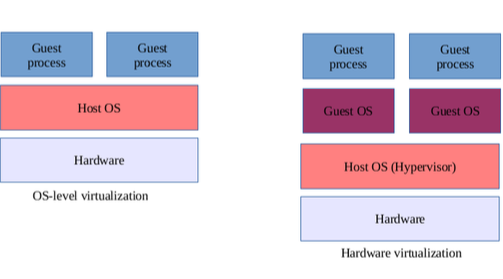
\includegraphics[width=0.7\textwidth]{gfx/examples/os_virt_diff}
 \caption{Architectural difference container and full virtualization}
 \label{fig:intro:diff_container_vm}
\end{figure}
Full virtualization allows it to run an entire guest operating system in a virtual machine (VM) on a host operating system. 
This is possible through an installed piece of software called hypervisor which is build classically on top of the originally operating system. 
This virtualization model provides solid security through this additional isolation layer. 
One obvious drawback is the heavyweight and high resource usage characteristic.
In contrast to classical virtualization a container does not need an additional operating system layer as seen in Figure \ref{fig:intro:diff_container_vm}. 
The container is just using and sharing the underlying kernel from the host. 

Containerization technology is closer to the underlying host operating system than the classical virtualization strategy. 
That makes containers more lightweight and flexible. 
Comparisons between container concepts and classical virtualization with regard to the application purposes are described in \cite{7921010}
The next section offers a closer look at containerization paradigm itself.



%*************************************************************************
% Containerization
% ***
\section{Containerization paradigm}
\label{sec:intro:containerization}
%Definition Container
% Short overview of how a container works
% Short architecture
% properties
%
% 
In theory the paradigm of containers is very simple. 
Containers are basically operated as stateless and separate units. 
These units can fulfill certain tasks by acting autonomously as isolated software components.
The paradigm is integrated by certain kernel functionalities. 
These functionalities with the jails concept in BSD have been introduced in the early 2000s \cite{Souppaya:2017aa}.
In 2008 more functionalities have been popularized in a user-friendly way in the Linux kernel.
The framework is called Linux Containers(LXC's) \cite{Souppaya:2017aa}.
However the usage of LXC's can become quite complex.
The using of LXC has become much easier since Docker was introduced as a wrapper.
Docker offers a user-friendly interaction with the LXC framework and has established itself as a state-of-the-art construct in terms of containerization.
Nowadays developers are able to provide containers due to Docker at a much faster pace than with pure LXC's. 
	
Native Linux features are responsible for the encapsulation between host and deployed containers.

Since the introduction of container technology under BSD, native functions form the basic framework of containers.
These necessary isolation and permission concepts are described in the following.

%*************************************************************************
% Linux namespaces
% ***
\section{Linux namespaces}
\label{sec:intro:containerization:linux_namespaces}
A Linux namespace encloses a global system resource in an abstraction that makes the processes within the namespace appear to have their own isolated instance of the global resource. Changes to the global resource are visible to other processes that are members of the namespace, but invisible to other processes. Namespaces are the basic building block of containers under Linux. The following namespaces exist under Linux:
\begin{itemize}
\item Cgroup
\item Interprocess communication (IPC)
\item Network
\item Mount
\item PID
\item User
\item UTS
\end{itemize}
Unfortunately it is utopian to describe every namespace type in depth in this work. 
The IPC and mount namespace are described now briefly. Then the more interesting namespaces are explained in a dedicated subsection.

Mount namespaces provide an isolation of the list of mount points seen by the processes in each namespace instance. Processes in each of the mount namespace instances see different single views of directory hierarchies. This view can range from physical or network drives, mount paths or advanced features such as union file systems which are discussed in section \ref{sec:intro:docker_image:unionfs}.

IPC namespaces isolate certain IPC resources like System V IPC objects and POSIX message queues which both are data structures they allow via e.g. shared memory to transfer information between processes.

\subsection{PID}
\label{sec:intro:containerization:linux_namespaces:pid_namespaces}
Traditionally the Linux kernel has always maintained a single process tree. The tree contains a reference to each process currently running in a parent-child hierarchy. 
A Linux system starts with process PID1. This is the root of the process tree and the root process initiates the rest of the system by starting different handlers and services. All other processes start below this process PID1 in the tree. 

The basic idea behind PID namespaces is to create and append a new root tree to the already existing tree with its own PID1. This makes the child process to a root process.
Processes in the subordinate namespace have no way to detect the existence of the parent process. This ensures that processes that belong to a process tree do not inspect or kill processes in other process trees. However processes in the higher-level namespace have a full view in the lower-level namespace of processes.

\subsection{Network}
\label{sec:intro:containerization:linux_namespaces:network_namespaces}
Due to the global instance of the network interface on a single host it is possible with granted permissions to alter routing and ARP tables. With network namespaces totally different instances of network interfaces can be provided. Routing and ARP tables then operate independent of each other. This prevents communication between network namespaces.
 
Network namespaces are complex but important to know. These are responsible to establish communication between containers and hosts and between containers themselves. 
The following enumeration shows the standardized CNI (Container Network Interface) workflow. CNI describes how network namespaces are created and how a desired communication between these namespaces can be established.

\begin{enumerate}
\item Create network namespace
\item Create bridge network/interface
\item Create virtual-ethernet pairs
\item Attach virtual-ethernet to namespace and bridge
\item Assign IP addresses
\item Bring interfaces up
\end{enumerate}
For a better understanding an example with 2 network namespaces is shown in Figure \ref{sec:intro:containerization:linux_namespaces:netowork_ns}. Each color represents a network namespace with its associated virtual network interface pairs(veth-x and veth-x-bridge). For simplicity IP addresses are not shown. In this picture C1 is just a prefix for the underlying hostname which is arbitrary in this case. Basically communication between any networks from a view of a network namespace is not possible as already mentioned. Network communication between namespaces is allowed after the CNI procedure. Finally the two interface endpoints (purple and orange) have a valid IP address which leads to a working network communication.
\begin{figure}[htbp]
 \centering
 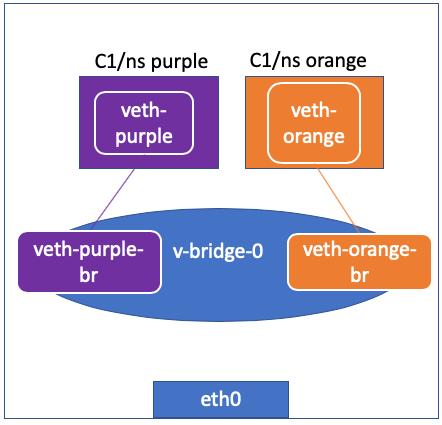
\includegraphics[width=0.4\textwidth]{gfx/examples/network_ns}
 \caption{Example of basic network within a container cluster}
\label{sec:intro:containerization:linux_namespaces:netowork_ns}
\end{figure}
This is the beginning of network communication through namespaces and CNI. However only inter communication between different namespaces on a single host is not sufficient. Several steps are required to communicate externally to other host and across the Internet.

Figure \ref{sec:intro:containerization:linux_namespaces:netowork_ns_out} shows a more comprehensive setup. 
It shows that the local host is also the gateway because it has one network connection through the interface eth0 and it has access to the bridge network created on the host. 
A routing table entry in the blue network namespace like the following necessary, if the blue namespace network needs to access the endpoint with the IP address 192.168.1.3 
\begin{lstlisting}
	ip netns exec blue ip route add 192.168.1.0/24 via 192.168.15.5
\end{lstlisting}
This allows the direction from the namespace to the outside endpoint. To enable access from outside to this network namespace it is necessary to create a NAT rule via iptables.
\begin{lstlisting}
	iptables -t nat -A POSTROUTING -s 192.168.15.0/24 -j MASQUERADE	
\end{lstlisting}
In order to provide access to the internet from a namespace it is necessary to add a default route as seen below.
\begin{lstlisting}
	ip netns exec blue ip rout add default via 192.168.15.5
\end{lstlisting}
\begin{figure}[htbp]
 \centering
 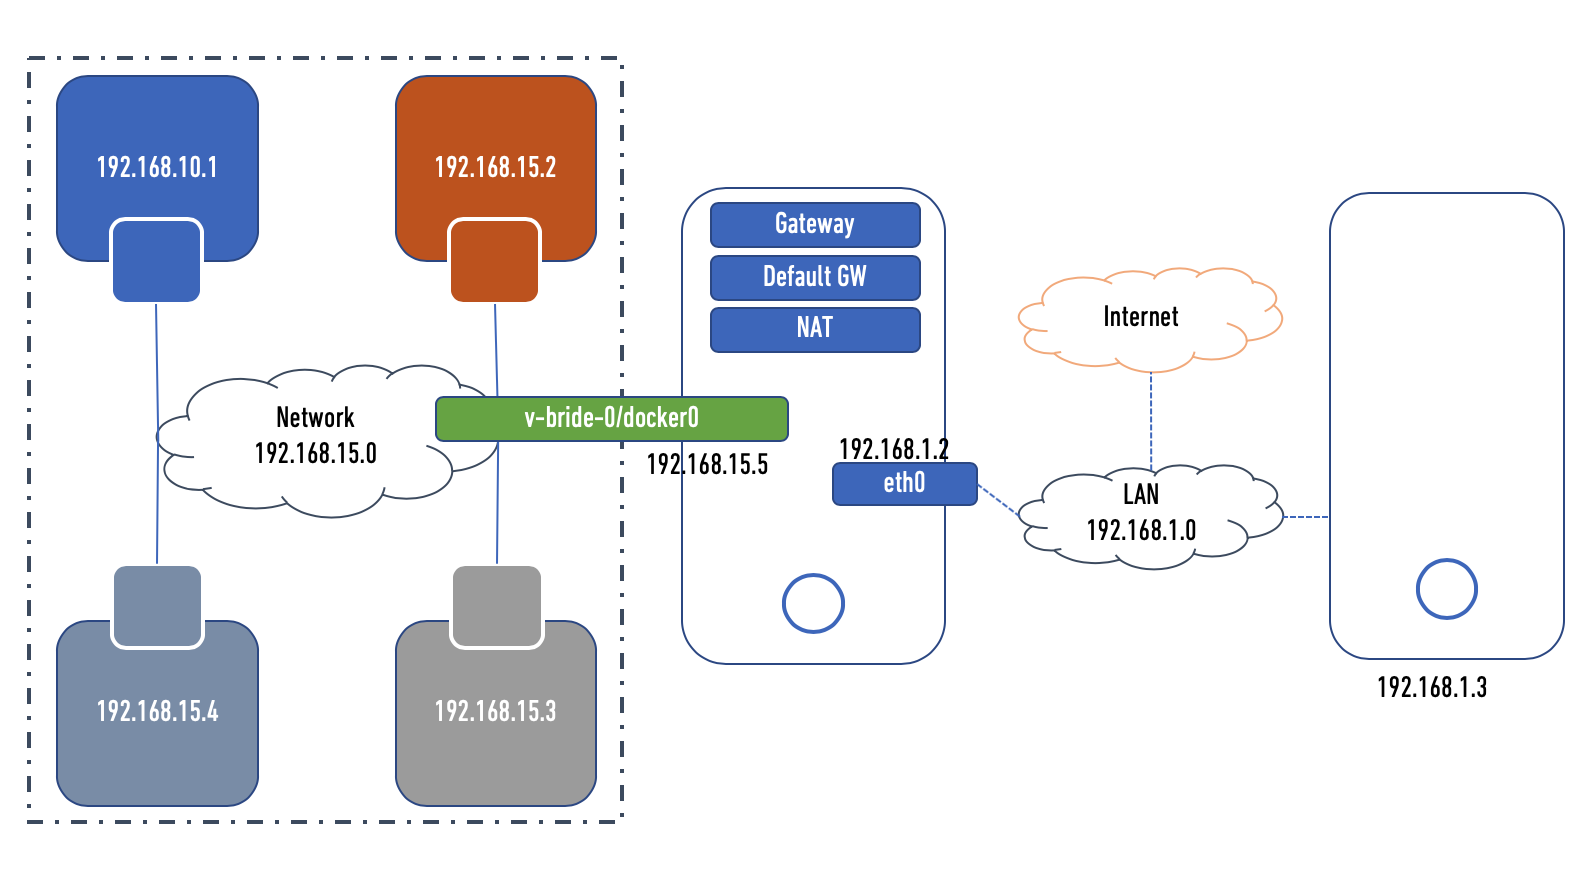
\includegraphics[width=0.7\textwidth]{gfx/examples/network_ns_out}
 \caption{Example of comprehensive networking within and outside of container}
\label{sec:intro:containerization:linux_namespaces:netowork_ns_out}
\end{figure}
This example of network namespaces demonstrates the power and flexibility of network namespaces.
Normally these steps are automatically done through a container daemon like Docker. This in turn can also be managed by an orchestrator like Kubernetes or Mesos.

Lastly the user namespace is left and described in the following.

\subsection{User}
\label{sec:intro:containerization:linux_namespaces:user_namespaces}
User namespaces isolate user and group IDs so that they appear differently in and outside the user namespace.
User namespaces give processes the ability to believe that they are working as root when they are inside the namespace.
User namespaces can also operate on capabilities. 

What are capabilities? In contrast to privileged processes that bypass all kernel permission checks, unprivileged processes have to pass full permission checking based on the process’s credentials such as effective UID, GID and supplementary group list. Linux has privileged process rights divided into different units called capabilities. These distinct units/privileges can be independently assigned and enabled for unprivileged processes.

The next section describes in short another Linux kernel feature called cgroups. They provide another level of security in order to provide a smooth working container environment.

\section{Cgroups}
\label{sec:intro:containerization:cgroups}
Control groups (Cgroups) are a way of enforcing hardware resource limitations and access controls on a process or set of processes. The cgroup scheme provide a hierarchical, inheritable and optionally nested resource control mechanism.
In the world of containers Cgroups manifest themselves as instruments to prevent runaway containers and denial of service attacks.
The following enumeration contains the resources that are controlled by cgroups.
\begin{itemize}
\item CPU usage
\item Memory usage
\item Disk usages
\item Device whitelist
\item Network traffic based on tags(class id value) and iptables for filtering
\item Application freeze and unfreeze by sending special signals
\item PID limitation to limit a specific amount of processes 
\end{itemize}

After this section awareness is raised of the fact that containers work in isolation via native Linux functions.
The next important section gives an architectural introduction to the base of every container - a container image.



%*************************************************************************
% Union FS
% ***
\section{Unionfs}
\label{sec:intro:docker_image:unionfs}
This paper uses Docker as container technology as already mentioned in chapter \ref{ch:intro} .
To have knowledge of union file systems is necessary before delving into container and especially Docker image insights.
Union file systems build the basis for container images in general. This section explains one important file system - the Overlay2 file system.

A union file system represents a file system by grouping directories and files. There are several union file system available like BTRF, AUFS, ZFS and Overlay2 which are compared in detail in \cite{Tarasov2019}.
Only Overlay2 will be considered in this work because Overlay2 is directly implemented in the Linux kernel \cite{Tarasov2019} and is meanwhile the standard in Docker related to Docker Inc. \cite{docker_storage_driver}.
Basically Overlay2 needs at least 4 directory types to work correctly:
\begin{itemize}
\item Lower directory - usually read-only and can be an overlay itself
\item Upper directory - is normally writable
\item Merged directory - represents the union view of the lower and upper directory
\item Work directory - used to prepare files before they are switched to the overlay/merged destination in an atomic action 
\end{itemize}
The elements of an Overlay2 file system are now described with the help of an example. 
First the following folder structure in Listing \ref{intro:overlay:hierarchy} is assumed.
\lstinputlisting[caption={Tree orig}, captionpos=b, label={intro:overlay:hierarchy}]{chapters/intro/listings/tree1.txt}
The folder structure contains all the mandatory Overlay2 elements. The mount point can be created without additional software packages because Overlay2 is natively supported under Linux.
This is illustrated by the following mount command.
\begin{lstlisting}[label={intro:overlay:mountcmd}]
	mount -t overlay -o lowerdir=./lower1:./lower2,upperdir=./upper,workdir=./work overlay ./merged
\end{lstlisting}
First the command must know what type of file system to mount. This information is provided by the -t switch. In this case it is an overlay type. The next flag -o allows to add options to mount the specific filesystem. Each option with associated values is separated by a comma. The option lowerdir is set to a chain of folders separated by a colon. The lowerdir argument takes only the lower1 and lower2 directory. Then upperdir is set to the upper folder of the provided hierarchy. The worker option represents a single folder and is set accordingly to the worker folder. Lastly overlay option needs an argument to provide the union mount on the file system. This union view is presented through the merged directory.

The behavior of the Overlay2 file system is demonstrated in the following.
The file system as a whole is populated with files as seen in Figure \ref{sec:intro:docker_image:treefilled}.
\lstinputlisting[caption={Tree filled}, captionpos=b, label={sec:intro:docker_image:treefilled}]{chapters/intro/listings/tree2.txt}
A file creation in one of the lower- and upper directories is visible as expected in the merged directory.
A file or directory object in the upper directory tree appears in the overlay. The same object is not visible in the lower directory.
Each directory content is merged to create a combined directory object in the overlay.
A file or directory that originates from the overlay is removed from the overlay when it has been removed from the upper directory. 
A file or directory that originates from the lower directory remains in the lower directory when it was removed from the overlay-directory, but a 'whiteout' mark is created in the upper directory. A whiteout takes the form of a character device with device number 0/0 and a name identical to the removed object. A whiteout ensures that the object in the lower directory is simply ignored. Also a whiteout is not not visible in the overlay directory. 

Another important fact about union file system is the use of copy on write strategy. 
A storage driver manager takes care of copying files to the upper layer when a file from an underlying layer has been modified. A duplicate is created and the modification takes place. This is an efficient resource management technique because operations may just need a copy instead of creating a new file.
	
The general knowledge about the Overlay2 file system is provided. This is important to understand the main component - the Docker image. This is described in the following.

%*************************************************************************
% Docker image
% ***
\section{Docker image}
\label{sec:intro:docker_image:docker_img}
In this section, the Docker image is explained in more detail, as it is an important part of the work. First, the architecture of a Docker image is presented with the necessary information for further work, since the overall architecture with all information would make the basic chapter too large. Then the construct for building a Docker image is explained. This is called Dockerfile and in the introduction the key factors and usage of Dockerfile is explained. 
Finally, the last subsection describes the metadata information, as it is important to follow the theoretical concept.

\subsection{Docker Image architecture}
\label{sec:intro:docker_image:docker_img:architecture}
A Docker image is ultimately a stack of selected file system layers to provide a starting point for a container.
Fig \ref{sec:intro:docker_image:docker_image_stack} shows how a Docker image is stacked. At the bottom there is the Linux kernel. On top of that takes two different image layers place. In this case it is a Debian and a Busybox.
Both of them are runnable base images.
On top of these layers can be more layers stacked as shown on the Debian layer with an additional Emacs and an Apache layer. The busybox itself doesn't have another further layer stacked on the top.
When a container is launched from an image, Docker finally attaches a read/write file system across all underlying layers, as it is seen on both images in this example.

\begin{figure}[htbp]
 \centering
 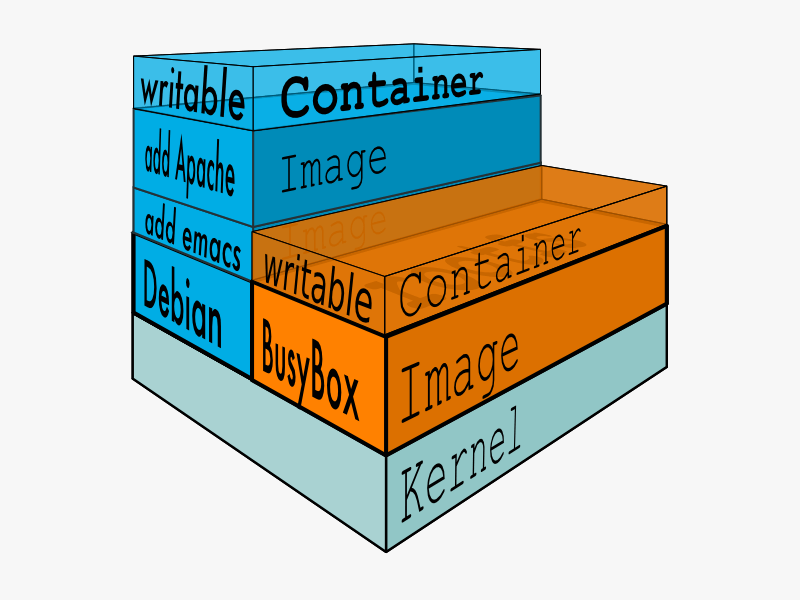
\includegraphics[width=0.6\textwidth]{gfx/examples/docker-filesystems-busyboxrw}
 \caption{Docker filesystems stacked to represent an image}
\label{sec:intro:docker_image:docker_image_stack}
\end{figure}

In order to manage images and especially corresponding file system layers, Docker uses storage drivers. Each storage driver handles the implementation differently.
There are several storage drivers available like, ZFS, BTRFS and many more which can be configured by the responsible system-engineer or developer. Docker uses in the latest version Overlay2 as storage driver per default. The Overlay2 informations about an image can be viewed by the Docker inspect command.
\begin{lstlisting}
	docker inspect ubuntu
\end{lstlisting}

The inspection provides a result tailored to show only filesystem level information, as this is the interesting part for the docker architecture.
 
\lstinputlisting[caption={Docker inspection results}, firstline=71, lastline=79, captionpos=b, label={sec:intro:docker_image:corresponding_unionfs}]{chapters/intro/listings/inspect_results.txt}

As seen in listing \ref{sec:intro:docker_image:corresponding_unionfs}, the introduced mechanisms of the Overlay2 union file system \ref{sec:intro:docker_image:unionfs} are used in order to provide a starting point for a container.
Each component of Overlay2 is found and is used by Docker. This represents once more, that Docker is using only Linux well known core functions instead of building own mechanisms.

One interesting and important fact is the mount process. The lower-directories which represents a readonly structure are not mounted directly by their folder name. Docker uses for each image layer a symbol link, which redirects to the original folder. The reason belongs only to the length of the folder name, which is in total a length of 65. These symbolic links help avoid the Linux ‘mount’ command from exceeding page size limitation.
It is also important to note that the \textbf{diff} directory in each layer builds the chain of the overlay. That can be seen in listing \ref{sec:intro:docker_image:corresponding_unionfs} as well. In each layer are additional helper files available like the lowerfile, which creates a relation to associated parent, if a parent exist.
The lower files are responsible for creating the correct order from the most upper layer to the lower layers. Due to this fact will be a correct order provided, since it is necessary for a correct behavior of a union file system.

Furthermore, every image has a name and a tag. An image name is made up of slash-separated name components, optionally prefixed by a registry hostname. The hostname must comply with standard DNS rules, but may not contain underscores. A tag name must be valid ASCII and may contain lowercase and uppercase letters, digits, underscores, periods and dashes. A tag name may not start with a period or a dash and may contain a maximum of 128 characters.
It is important to know that the name and the tag are separated by a colon.
This knowledge about the naming and tagging connection is helpful, since it finds application in the following chapters. The next section describes the construct of building a Docker image, called Dockerfile.

\subsection{Dockerfile}
\label{sec:intro:docker_image:docker_img:dockerfile}
In order to build a Docker image, Docker Inc. introduced a construct called Dockerfile.
Each entry in this Dockerfile starts with a keyword. These keywords can be used by a developer to assemble an image. Each entry in a Dockerfile creates a different file system layer. In other words each file system layer represents an instruction with help of a keyword in a Dockerfile.
The Dockerfile construct provides around 20 keywords \cite{dockerfile_ref}.
The following listing in \ref{sec:intro:docker_image:dockerfile} shows a typical Dockerfile.
\lstinputlisting[caption={Dockerfile}, captionpos=b, label=sec:intro:docker_image:dockerfile]{chapters/intro/listings/dockerfile.txt}
The FROM statement starts out by creating a layer from the ubuntu:18.04 image. The COPY command adds an example bash script from the Docker client’s current directory. The RUN command makes the program executable. Finally, the last layer specifies which command will be executed inside the container.

An image can be created with the corresponding Dockerfile and the command Docker build, like it is shown below.
\begin{lstlisting}
	docker build <my_new_image> -f <dockerfile>
\end{lstlisting}
It is valuable to know the Dockerfile construct, because it is finally responsible for integrating secrets into an image. 
From a logical view, there are two categories in a Dockerfile which contain commands that are responsible for integrating static files.
First, \textit{direct integration} which contains the actions COPY and ADD. The difference between the two commands lies in the range of functions. ADD can as an example request an URL or unzip an archive directly to the endpoint.

The second category \textit{indirect integration} is a bit more comprehensive. This category contains the action RUN.
Docker itself uses RUN to trigger a shell command and commit it to a new image layer.
The executed shell commands for RUN are inline defined. That allows cases, loop-constructs and external program execution. A flexible bunch of code is allowed, since it is just standard bash. This allows a developer to use available tools like ssh-keygen, openssl and manual file and folder creation. It is totally up to the developer what do to with that inline command in the Dockerfile. 


At this time it is known what a Docker image is and how it can be built. Also, it is known to integrate static files into an image in an indirect and direct way.  The next subsection will introduce the important topic metadata of an image which will be definitely used in the following chapters. 

\subsection{Docker Metadata}
\label{sec:intro:docker_image:docker_img:meta}
Another important feature is the metadata of an image. Every Docker image contains several meta-information of the build process. These meta-informations are directly accessible through the history feature. 
These informations are locally provided and accessible for the root user. 
It is assumed in this work that no manipulation of the metadata was performed locally. An integrity check would be desirable and need further investigation.

Using Ubuntu 18.04 as an example, the meta-information looks like this below \ref{sec:intro:docker_image:meta}:
\lstinputlisting[caption={Prototype structure in Python}, captionpos=b, label={sec:intro:docker_image:meta}]{chapters/main/practical/listings/meta.txt}
This listing might be confusing but it is helpful to just get an overview how it is structured, and how it can be helpful for the next chapters.
It can be seen that the schema of this meta information is similar to JSON. The only difference is that numeral values are not marked in quotations. In this structure there are many attributes with their corresponding values. Attributes like "Created", "CreatyBy" are first followed by "Id" and many more. 	
Important informations are most of all Dockerfile instructions like COPY, ADD an RUN, since they are responsible for integrating static files into the image.
In this example it can be seen that only an ADD command is used. A COPY method is not used.
A special fact applies to the RUN command. RUN commands are not directly listed in the meta informations.
Instead, only the executable command that follows a RUN command is visible.

In theory it is easy to analyse these informations because it is readable for computers because of the javascript object notation similarity.
That makes this history feature of Docker very important especially when it comes to the (pre-)processing of Docker images.	 Important properties can be extracted, such as Dockerfile keywords and corresponding parameters.

This chapter provided a basic knowledge about the architecture Docker images and the interaction with Overlay2. This knowledge is fundamental to have an idea how the file structure is working behind the scenes. It gives some ideas for the theoretical concept to analyse such an image for static secrets.
Before this is possible some related work is shown about key leak techniques. Key leak techniques are essential in order to detect secrets.

















